With the rise of General-Purpose Graphics Processing Unit (GPGPU) computing and
compute-heavy workloads like machine-learning, compute accelerators have become
a necessary component in both high-performance supercomputers and
datacenter-scale systems. The first exascale machines are expected to heavily
leverage the massively parallel compute capabilities of GPUs or other highly
parallel accelerators \cite{snl_roadmap}. As the software stack and programming model of GPUs and
their accelerator peers continue to improve, there is every indication that
this trend will continue. As a result, architects that wish to study the design
of large-scale systems will need to evaluate the effect that their techniques have
using a GPU model. However, the focus of all publicly available cycle-level
simulators ({\em e.g}GPGPU-Sim \cite{gpgpu_sim}) to date, has been on single-node
simulation performance. In order to truly study
the problem at scale, or for the simulation of large workloads, a parallelizable,
multi-node GPU simulator is necessary.

   \begin{figure}[!htb]
      \centering
      \setlength{\abovecaptionskip}{6pt plus 1pt minus 1pt}
      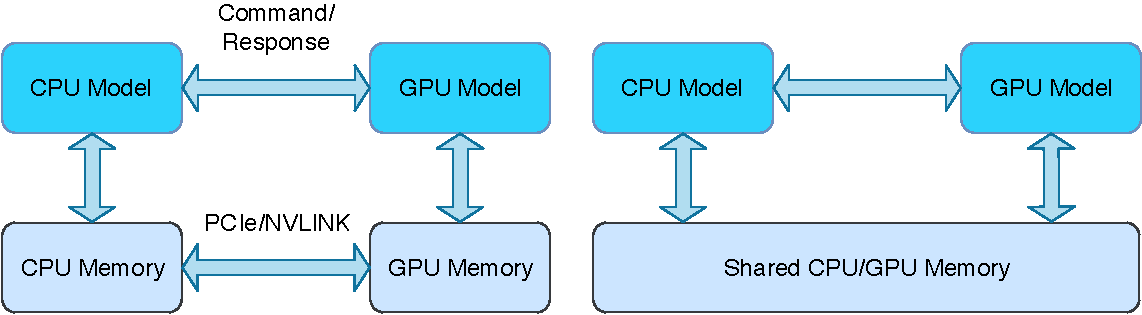
\includegraphics[width=.85\textwidth,keepaspectratio]{figures/cpu_gpu_model.pdf}
      \captionsetup{width=.75\textwidth}
      \caption{High-level CPU/GPU interaction model}
      \label{fig:model}
   \end{figure}

Figure~\ref{fig:model} depicts the current CPU/GPU model co-processor model.
On the left is the common high-performance, discrete GPU configuration, where the CPU
and GPU have separate memory spaces and are connected via either PCIe or a
high-bandwidth link (such as NVLink). The right shows an Accelerated Processing Unit (APU
 model where the CPU
and GPU share a single memory. Note that in even in the discrete memory case, modern
memory translation units allow the CPU and GPU to share the same virtual address space,
although the memories themselves are discrete components.

In this report we will detail a model that is capable of simulating both
discrete and unified memory spaces by leveraging the MemHeirarchy interface in
SST \cite{sst}. This report details our efforts to integrate the functional and streaming
multiprocessor core models from the open-source simulator GPGPU-Sim into SST.
